\section{EXPERIMENTS} \label{sec:experiments}

In this section we present numerical results of the validation benchmark and
  discuss a proof of concept application in the domain of particle
  accelerators.

\subsection{Optimizer Validation}

\begin{figure}
    \centering
    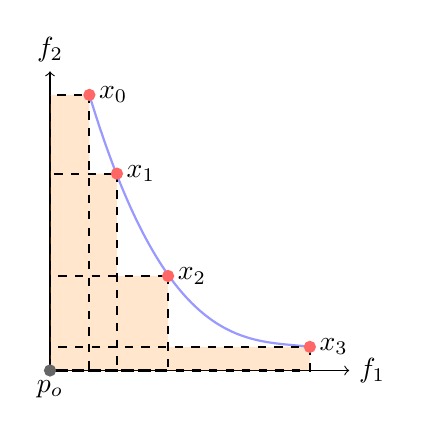
\begin{tikzpicture}[text=black]
      \coordinate (y) at (0,3.8);
\coordinate (x) at (3.8,0);
\draw[<->] (y) node[above] {$f_2$} -- (0,0) --  (x) node[right]
{$f_1$};

\path
  coordinate (start) at (0.5,3.5)
  coordinate (c1) at +(1.5,0.2)
  coordinate (c2) at +(2.5,0.4)
  coordinate (top) at (3.3,0.3);

\draw [thick, blue!40!white] (start) .. controls (c1) and (c2) .. (top);
(start) .. controls (c1) and (c2) .. (top) -- (3.3,0.0);
%\draw [fill, color=blue, draw opacity=0, fill opacity=0.2] (0,0) -- (0.0, 3.5) --
%(start) .. controls (c1) and (c2) .. (top) -- (3.3,0.0);


\draw[fill, color=orange, draw opacity=0, fill opacity=0.2] (0,0) -- (0, 3.5) --
(start) -- (0.5,2.5) -- (0.85, 2.5) -- (0.85, 1.2) -- (1.5, 1.2) -- (1.5, 0.3) -- (top) -- (3.3, 0.0);
\draw[dashed, thick] (start) rectangle (0,0);
\draw[dashed, thick] (top) rectangle (0,0);
\draw[dashed, thick] (0.85,2.5) rectangle (0,0);
\draw[dashed, thick] (1.5,1.2) rectangle (0,0);

\filldraw [red!60!white]
(start) circle (2pt) node[right, black] {$x_0$}
(0.85,2.5) circle (2pt) node[right, black] {$x_1$}
(1.5,1.2) circle (2pt) node[right, black] {$x_2$}
(top) circle (2pt) node[right, black] {$x_3$};

\filldraw [black!60!white]
(0,0) circle (2pt) node[below, black] {$p_o$};


    \end{tikzpicture}
  \caption{The hypervolume for a two-objective optimization problem
  corresponds to the shaded area formed by the dashed rectangles spanned by
  all points on the Pareto front and an arbitrary selected origin $p_o$.}
  \label{fig:hypervolume}
\end{figure}

To ensure that the optimizer works correctly we solved the benchmark
  problem (\ref{eqn:bench}).
To that end, we use a metric for comparing the quality of a Pareto
  front.
Given a point in the Pareto set, we compute the $m$ dimensional volume (for
  $m$ objectives) of the dominated space, relative a chosen origin.
We visualize this for $2$ objectives in Figure~\ref{fig:hypervolume}.
For further information and details of the implementation see~\cite{whbb:12}.
Figure~\ref{fig:pisa_bench} and the corresponding hypervolume values in
  Table~\ref{tbl:bench_rms_error}.
The reference Pareto front is clearly very well approximated.
It took a total of 1100 function evaluations to perform this computation.
The hypervolume of the reference solution ($0.6575$) for our benchmark was
  computed by sampling the solution provided in~\cite{hbwh:05}.

\begin{figure}
  \centering
    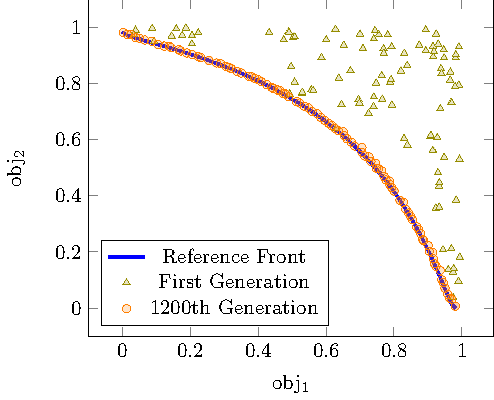
\includegraphics[width=0.7\linewidth]{figures/valid_front}
  \caption{Variator benchmark after $1100$ function evaluations using binary
           crossover and independent gene mutations (each gene mutates with
           probability $p=\frac{1}{2}$) on a population of $100$
           individuals.}
  \label{fig:pisa_bench}
\end{figure}

\begin{table}%[h!]
\begin{center}
  \caption{Convergence of benchmark problem with errors relative to
    hypervolume of sampled reference solution.}
  \label{tbl:bench_rms_error}
  \begin{tabular}{lcc}
    \hline\noalign{\smallskip}
    tot.\ function  & hyper volume & relative error\\
    evaluations    & & \\
    \noalign{\smallskip}\hline\noalign{\smallskip}
    100  &  0.859753 & $3.076 \times 10^{-1}$ \\
    \noalign{\smallskip}\hline\noalign{\smallskip}
    200  &  0.784943 & $1.938 \times 10^{-1}$ \\
    500  &  0.685183 & $4.210 \times 10^{-2}$ \\
    900  &  0.661898 & $6.689 \times 10^{-3}$ \\
    1100 &  0.657615 & $1.749 \times 10^{-4}$ \\
    \noalign{\smallskip}\hline
  \end{tabular}
\end{center}
\end{table}

From Table~\ref{tbl:bench_rms_error} we deduce that we achieved satisfactory
  convergence to the sampled reference Pareto front after 1000 (plus the
  additional 100 evaluations for the initial population) function evaluations.


\subsection{Ferrario Matching Point}\label{ferrario}

As a verification and proof of concept we reproduce the Ferrario
  matching point discovered by Ferrario \textit{et~al.}~\cite{fcpr:00},
  by formulating the problem as a  multi-objective optimization problem.
Using the low-dimensional and fast nature of their new simulation code
  Homdyn~\cite{homdyn}, an extensive beam dynamics study was conducted.

One of the results of the study presented in \cite{fcpr:00} was the discovery
  of a novel working point.
The authors noticed that the second emittance minimum can profit from the
  additional emittance compensation in the accelerating traveling wave
  structure ensuring that the second emittance minimum occurs at a higher
  energy.
This property is attained if the beam emittance has a maximum and the root
  mean square (rms) beam size has a minimum at the entrance of the first
  accelerating traveling wave structure.
This behavior is illustrated in Figure~\ref{fig:fer_match}.

\begin{figure}
  \centering
  
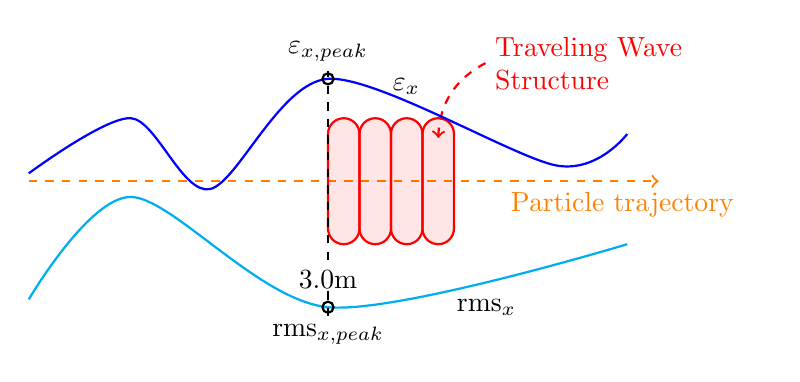
\begin{tikzpicture}

  \draw[dashed, thick, color=orange] (1.2,2.0) edge[->] (9.2,2);
  \node[orange, right, text width=3.2cm] at (7.2, 1.7) {Particle trajectory};

  %\draw[thick] (1.2,2.5) edge (9,2.5);
  %\draw[thick] (1.2,1.5) edge (9,1.5);
  %\node[above] at (1.0, 1.45) {Beam pipe};

  \draw[thick,color=red, fill=red, fill opacity=0.1, rounded corners=2mm] (5.0,1.2)
      rectangle (5.4,2.8);
  \draw[thick, dashed] (5.0,1.0) edge (5.0,3.4) node[below] {$3.0$m};
  \draw[thick,color=red, fill=red, fill opacity=0.1, rounded corners=2mm] (5.4,1.2)
      rectangle (5.8,2.8);
  \draw[thick,color=red, fill=red, fill opacity=0.1, rounded corners=2mm] (5.8,1.2)
      rectangle (6.2,2.8);
  \draw[thick,color=red, fill=red, fill opacity=0.1, rounded corners=2mm] (6.2,1.2)
      rectangle (6.6,2.8);
  \node[right, red, text width=2.8cm] at (7.0, 3.5) {Traveling Wave Structure};
  \draw[dashed, thick, color=red, bend right] (7.0,3.5) edge[->] (6.4,2.55);

  \draw[thick, cyan] plot [smooth, tension=0.5] coordinates {
      (1.2,0.5)
      (2.5,1.8)
      (5.0,0.4)
      (8.8,1.2)};
  \draw[thick, dashed] (5.0,0.6) edge (5.0,0.2);
  \draw[thick] (5.0,0.4) circle (2pt);
  \node[very thick, right] at (6.5, 0.4) {rms$_x$};
  \node[below] at (5.0, 0.3) {rms$_{x\text{, peak}}$};

  \draw[thick, blue] plot [smooth, tension=0.5] coordinates {
      (1.2,2.1)
      (2.5,2.8)
      (3.5,1.9)
      (5.0,3.3)
      (7.9,2.2)
      (8.8,2.6)};
  \draw[thick] (5.0,3.3) circle (2pt);
  \node[right] at (5.7, 3.2) {$\varepsilon_x$};
  \node[above] at (5.0, 3.4) {$\varepsilon_{x\text{, peak}}$};

\end{tikzpicture}

  \caption{Illustration of the Ferrario matching criteria: beam emittance
  attains a maximum and rms beamsize a minimum at the entrance to the first
  accelerating traveling wave structure.}
  \label{fig:fer_match}
\end{figure}

By artificially reproducing this working point as the solution of a
  multi-objective optimization problem given in equations
  (\ref{eq:swissfel:p1}) to (\ref{eq:swissfel:lastdvar}),
  we demonstrate the automation of discovering optimal beam dynamics behaviors
  given a set of desired objectives.

\begin{align}
  \text{min}  \quad & \left[ \Delta \text{rms}_{x,\text{peak}} = \vert 3.0 -
  \text{rms}_{x,\text{peak}} \vert, \right. \label{eq:swissfel:p1}\\
                    & \Delta \varepsilon_{x,\text{peak}}  = \vert 3.0 -
                    \varepsilon_{x,\text{peak}} \vert, \label{eq:swissfel:p2}\\
                    & \left. \vert \text{rms}_{x, \text{peak\_pos}} -
                    \varepsilon_{x,\text{peak\_pos}} \vert
                    \label{eq:swissfel:p3} \right]^T\\
  \text{subject to} \quad & q = 200 \left[\text{pC}\right] \label{eq:swissfel:firstconstr}\\
              \quad & \text{Volt}_{\text{RF}} = 100 \left[\text{MV/m}\right] \label{eq:swissfel:lastconstr}\\
              \quad & \sigma_{L} \leq \sigma_x = \sigma_y \leq \sigma_{U} \label{eq:swissfel:firstdvar}\\
              \quad & \text{KS}_{L} \leq \text{KS}_{\text{RF}} \leq \text{KS}_{U} \label{eq:swissfel:seconddvar}\\
              \quad & \text{LAG}_{L} \leq \text{LAG}_{\text{RF}} \leq \text{LAG}_{U} \\
              \quad & \Delta z_{L\text{KS}} \leq \Delta z_{\text{KS}} \leq \Delta z_{U\text{KS}} \label{eq:swissfel:lastdvar}
\end{align}

The first two objectives minimize the distance from the position of the current
  minimum peak to the expected peak location at $3.0$\,m for transverse bunch
  size (beam waist) and emittance (see Figure~\ref{fig:fer_match}).
The third objective (\ref{eq:swissfel:p3}) adds a condition preferring
  solutions that have their emittance and rms peak locations at the same
  $s$-coordinate.
Equations (\ref{eq:swissfel:firstconstr}) and (\ref{eq:swissfel:firstdvar})
  define constraints for initial conditions for the simulation: charge,
  gun voltage and laser spot size.
Design variables given in (\ref{eq:swissfel:seconddvar}) to
  (\ref{eq:swissfel:lastdvar}) correspond to field strengths of the
  first focusing magnet, its displacement, and the phase of the gun.

In order to compute the peaks, we employed an additional Python script.
This script was called in the \textsc{OPAL}~input file, after the simulation
  finished using the \texttt{SYSTEM} functionality.
Once the peaks (in a given range) were located, the two objectives
  (\ref{eq:swissfel:p1}) and (\ref{eq:swissfel:p2}) were computed and their
  values written into corresponding files.
The custom \texttt{fromFile} functor allows us to access the values stored in
  the peak finder Python script result files

\vspace{0.2cm}
{\footnotesize \begin{verbatim}
    rmsx:  OBJECTIVE, EXPR="statVariableAt("rms_x-err.dat", "var")";
    emitx: OBJECTIVE, EXPR="statVariableAt("emit_x-err.dat", "var")";
    match: OBJECTIVE, EXPR="fabs(statVariableAt("emit_x-peak.dat", "var") -
                                 statVariableAt("rms_x-peak.dat", "var"))";
\end{verbatim}}
\vspace{0.2cm}

\noindent
The design variables and the assembly of the multi-objective optimization problem
  can be included in the \textsc{OPAL}~input file as shown below:

\vspace{0.2cm}
{\footnotesize \begin{verbatim}
    d1:  DVAR, VARIABLE="SIGX", LOWERBOUND="0.00025", UPPERBOUND="0.00029";
    d2:  DVAR, VARIABLE="FIND1_MSOL10_i", LOWERBOUND="110", UPPERBOUND="120";
    d3:  DVAR, VARIABLE="D_LAG_RGUN", LOWERBOUND="-0.1", UPPERBOUND="0.1";
    d4:  DVAR, VARIABLE="D_SOLPOS", LOWERBOUND="-0.05", UPPERBOUND="0.05";

    objs:    OBJECTIVES = (rmsx, emitx);
    dvars:   DVARS = (d1, d2, d3, d4);
    constrs: CONSTRAINTS = ();
    opt:     OPTIMIZE, OBJECTIVES=objs, DVARS=dvars,
             CONSTRAINTS=constrs;
\end{verbatim}}
\vspace{0.2cm}

All numerical experiments in this sections were executed on the
  \textsc{Felsim} cluster at PSI\@.
The \textsc{Felsim} cluster consists of 8 dual quad-core Intel Xeon
  processors at 3.0 GHz and has $2$ GB memory per core with a total of 128
  cores.
The nodes are connected via Infiniband network with a total bandwidth of 16
  GB/s.

The envelope-tracker, mentioned in the previous section, was used to evaluate
  the forward problems.
We performed a beam convergence study in order to tune the simulation input
  parameters to achieve the best trade-off between simulation accuracy and
  time to solution.
These parameters include the number of slices (\texttt{NSLICE}) used in the
  envelope-tracker simulations, simulation timestep (\texttt{DT}) and gun
  timestep (\texttt{DTGUN}).

Before the simulation can be executed a number of initial beam optics
  parameters have to be defined in an input file.
Table~\ref{tbl:et_params} shows the values of these parameters for the
  envelope-tracker.
All simulations were performed up to 12.5~m of the
  \textsc{SwissFEL} 250 MeV injector~\cite{pedr:10} beam line, with
  energies reaching  up to 120 MeV.

\begin{figure}%[h!]
  \centering
  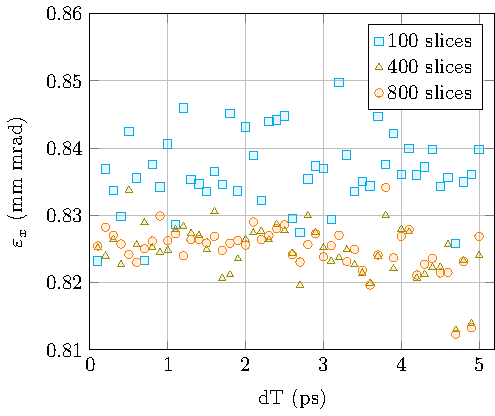
\includegraphics[width=0.8\linewidth]{Report/dt_scan}
  \caption{Envelope-tracker with different number of slices and simulation
    time steps.}
  \label{fig:et-dt}
\end{figure}

\begin{table}
  \begin{center}
    \caption{Initial conditions for the envelope tracker.}
    \label{tbl:et_params}
    \begin{tabular}{ll}
      \hline\noalign{\smallskip}
      name & initial value \\
      \noalign{\smallskip}\hline\noalign{\smallskip}
        Gun voltage       & $100$ MV\\
        %Solenoid current & $110.541$ A\\
        %Laser spot size  & $290 \times 10^{-6}$ m in x and y\\
        Bunch charge      & $200$ pC\\
        %DT$_{Gun}$        & $0.06$ ps\\
        DT$_{\text{Beamline}}$  & $1.5$ ps\\
        Number of slices  & $400$ \\
      \noalign{\smallskip}\hline
    \end{tabular}
  \end{center}
\end{table}

The parameter that affects the performance most is the number of slices.
We scanned the range from $100$ to $1000$ slices to determine the minimal
  number of slices required for stable results using various timesteps.
The results (for 100, 400 and 800 slices) of this scan are shown in
  Figure~\ref{fig:et-dt}.
Using this data we settled for $400$ slices -- increasing the slice number
  only minimally improves convergence of the results, therefore using more
  slices is inefficient.


%\begin{figure}
   %\centering
     %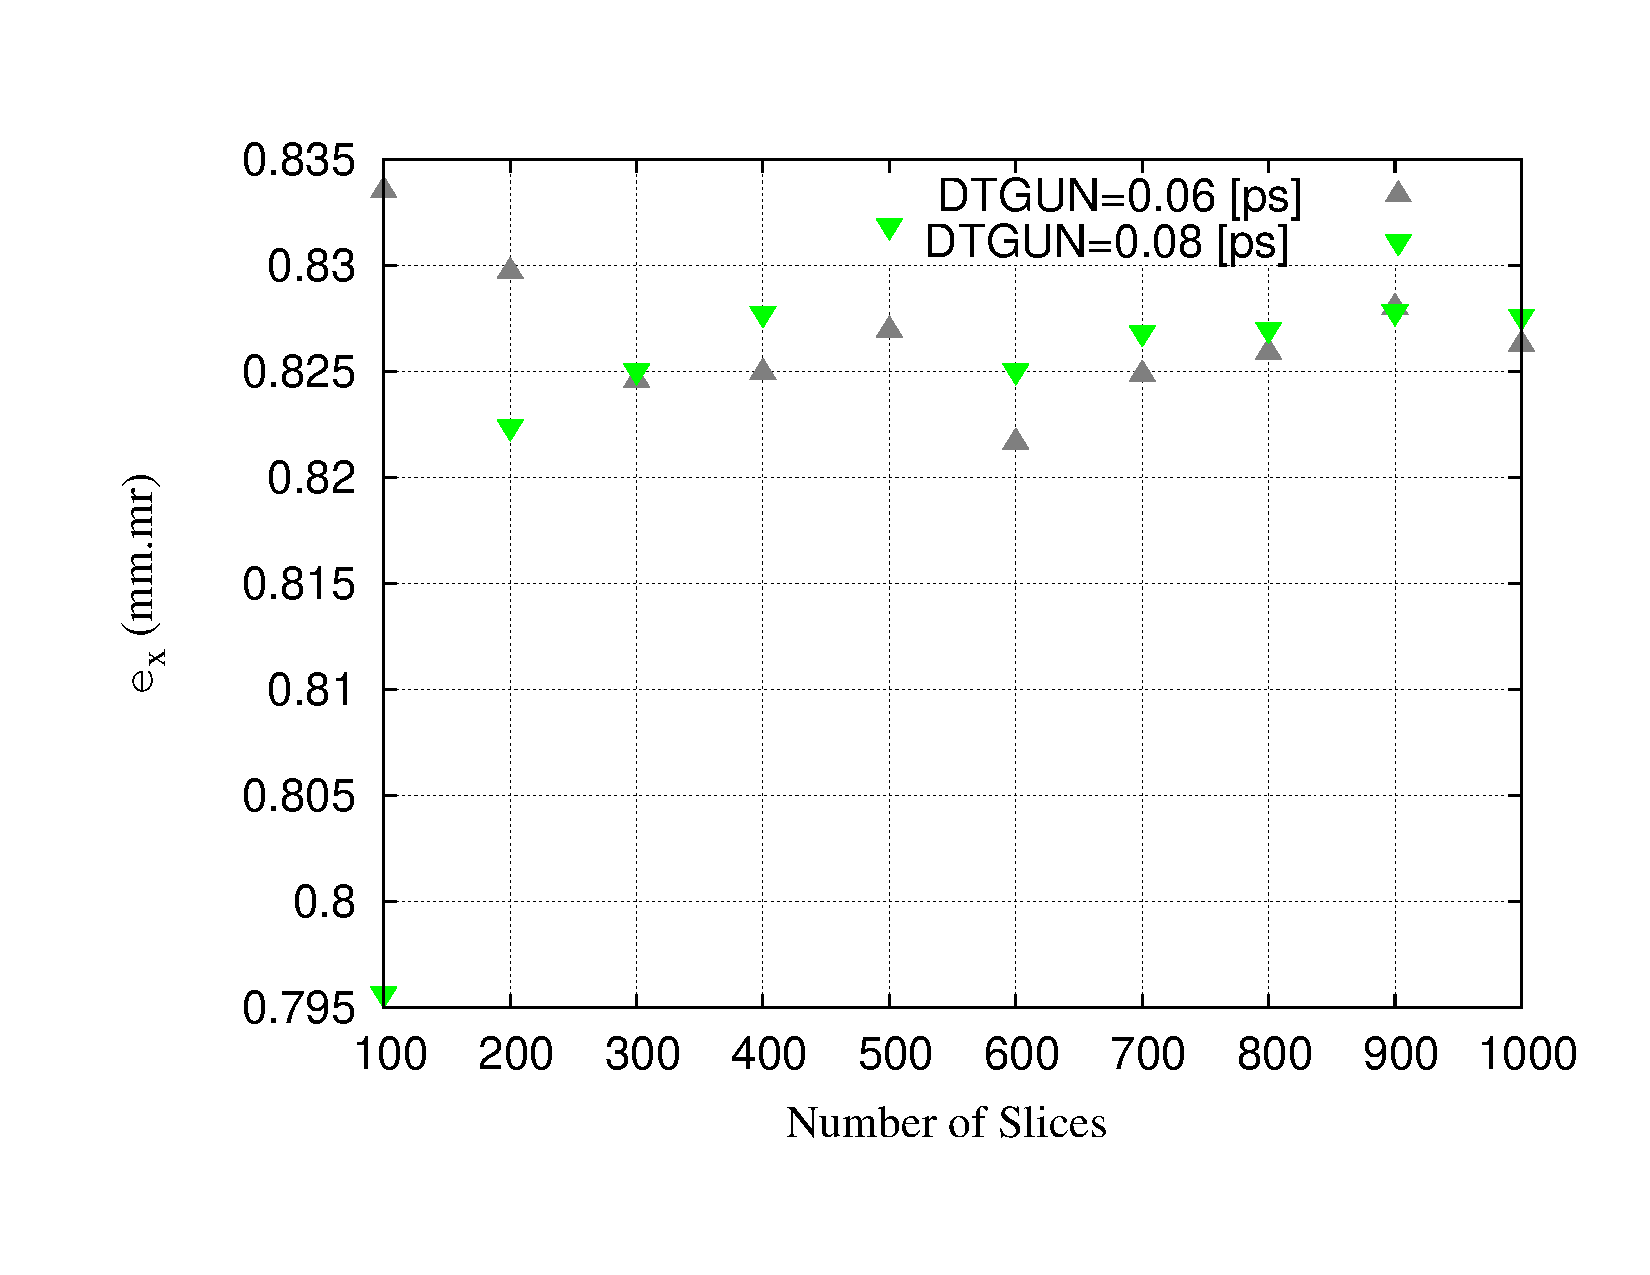
\includegraphics[angle=0,width=0.8\linewidth]{Report/sliceNew}
   %\caption{Scan of the envelope-tracker slice number showing its influence
            %on the exit emittance values.}
   %\label{fig:scan_slices}
%\end{figure}

In a next step the influence of different time steps was examined.
To that end a series of optimization runs with 100, 400 and 800 slices and
  varying timestep was performed.
%Figures \ref{fig:pareto_front_1} and \ref{fig:pareto_front_21} show two Pareto
Figure~\ref{fig:pareto_front_21} shows the Pareto fronts for 400 slices
  respectively using different timesteps.
As expected, increasing the number of slices while lowering the timestep
  produces more detailed results.

%\begin{figure}
  %\centering
    %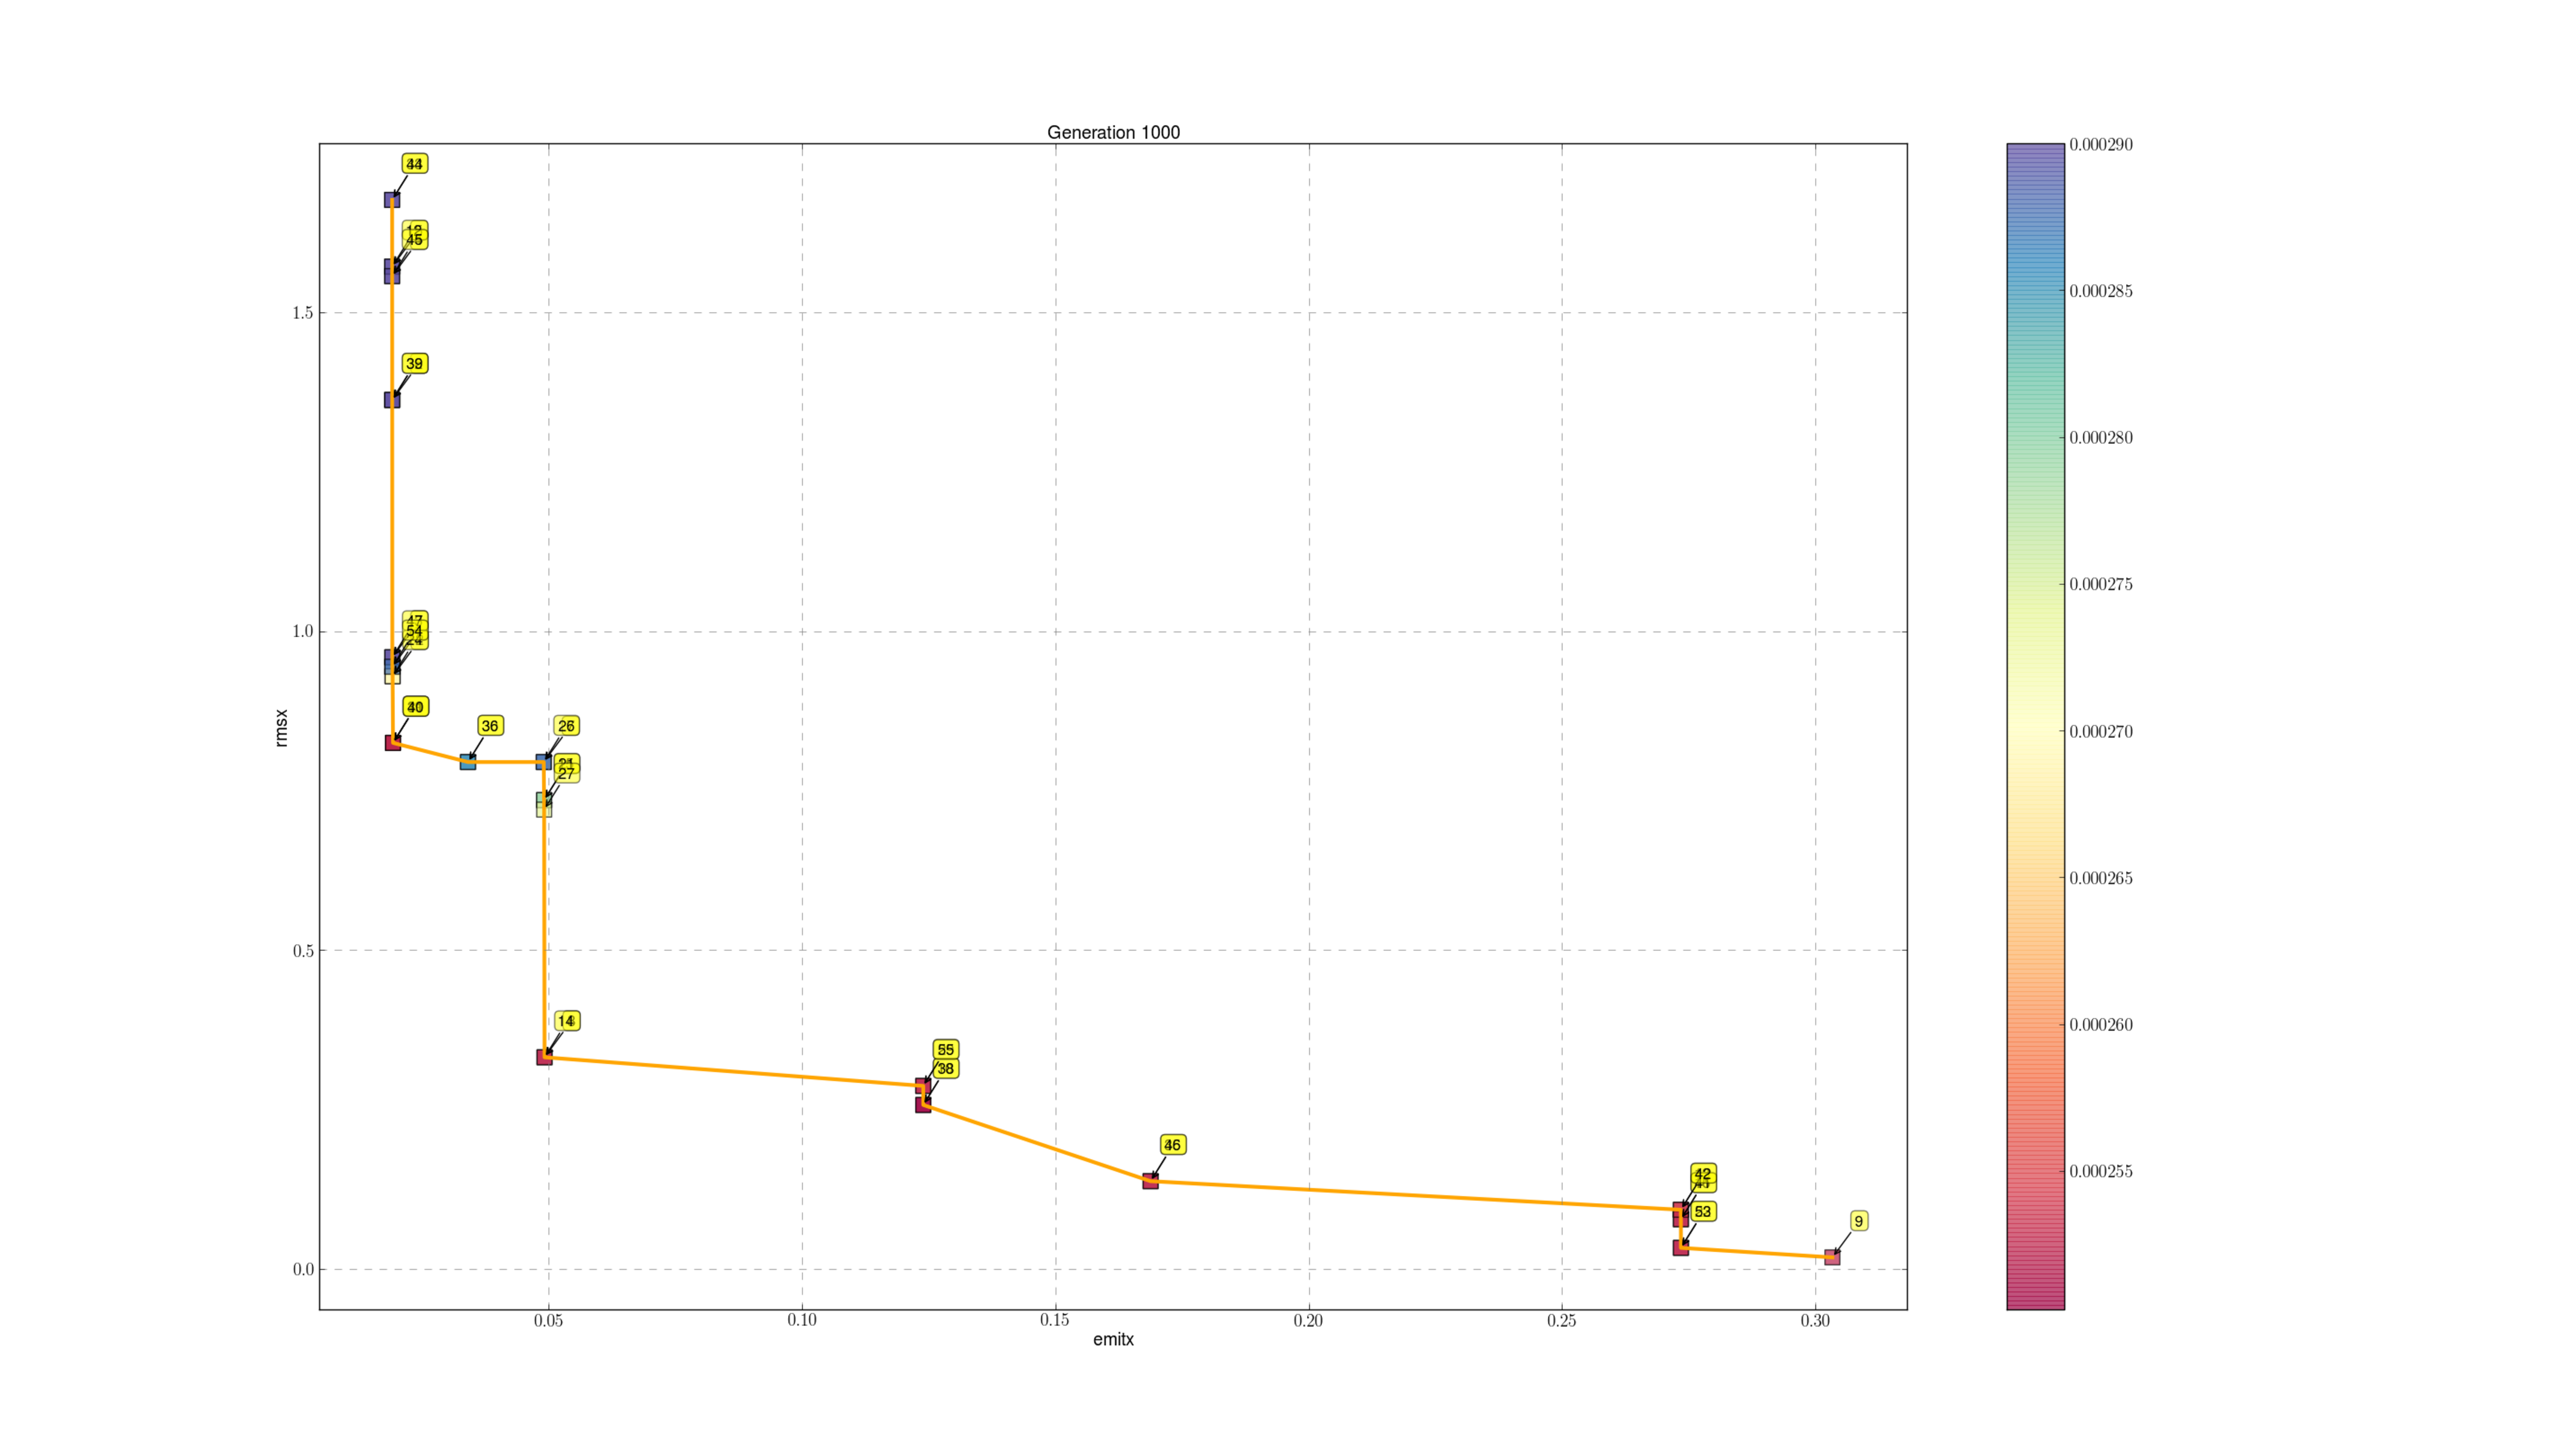
\includegraphics[width=0.9\linewidth]{Report/Run1slices100a}
  %\caption{Pareto Front for the $1000$th generation with $40$ individuals
    %using 100 slices, a simulation timestep of 5 ps and a gun timestep of 0.1
    %ps.}
  %\label{fig:pareto_front_1}
%\end{figure}

\begin{figure}%[h!]
  \centering
    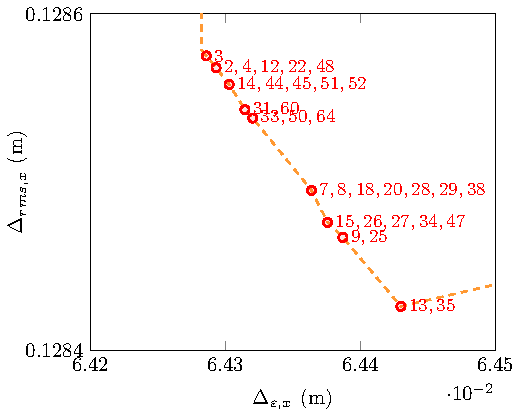
\includegraphics[width=0.8\linewidth]{Report/front_plot}
  \caption{Pareto front for the $1000$th generation with $40$ individuals
    using 400 slices (interesting region magnified), a simulation timestep
    of 1.5 ps.
    The individual 3 was selected for further investigations.}
  \label{fig:pareto_front_21}
\end{figure}


\subsubsection{Optimization Results}

Each of the $40$ points on the Pareto front, shown in
  Figure~\ref{fig:pareto_front_21}, represents an optimal solution, where
  emittance and beamsize values are compromised to achieve the best agreement
  with the Ferrario matching point.
We selected individual $3$ based on a comparison of the emittance and beamsize
  characteristics of all solutions and by retaining the feasibility of the
  beam line optics parameters.
The design variables, emittance and beamsize of the selected solution are
  shown in Table~\ref{tbl:des_vars} and Figure~\ref{fig:rmsemit}.
With the multi-objective optimization framework we attain the same working
  point as reported in~\cite{pedr:10}.

\begin{table}
  \begin{center}
    \caption{The design variables for individual $3$.}
    \label{tbl:des_vars}
    \begin{tabular}{ll}
      \hline\noalign{\smallskip}
      name & value \\
      \noalign{\smallskip}\hline\noalign{\smallskip}
        $\sigma_{x}$          & $0.262$ mm \\
        Solenoid displacement & $28.8467$ mm \\
        Gun voltage lag       & $0.0159067$ MV\\
        Solenoid current      & $111.426$ A \\
      \noalign{\smallskip}\hline
    \end{tabular}
  \end{center}
\end{table}

\begin{figure}%[h!]
  \centering
  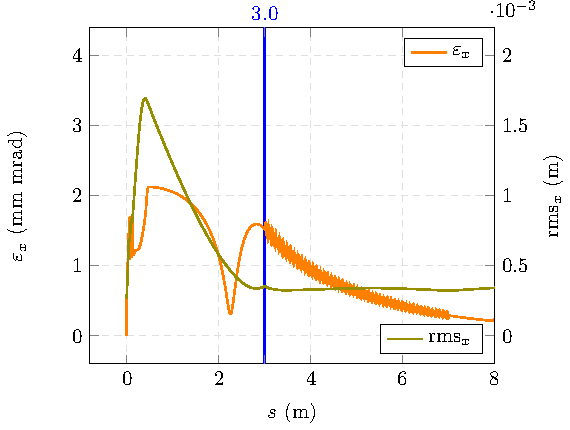
\includegraphics[width=0.8\linewidth]{Report/iff_plot_emrms}
  \caption{Beamsize and emittance of individual $3$.}
  \label{fig:rmsemit}
\end{figure}

Using the input parameters of the selected solution, we performed a stability
  analysis by varying the slice number and the time step for both the gun and
  the beam line.
Figure~\ref{fig:et-dt} shows that the exit emittance stabilizes for 400
  slices and various time steps.
No difference between $800$ and $400$ slices is visible as their minimum
  maximum extension seems to be in the same range of $0.024$ mm~mrad.

For validation purposes we compared the results of the envelope-tracker using
  the analytical space charge model with the \textsc{OPAL} 3D macro particle
  tracker.
The benchmark was run on the first 12.5 meters of the \textsc{SwissFEL} 250
  MeV injector.
The results for both rms beamsize and emittance are shown in
  Figure~\ref{fig:et-vs-tt}.
A good agreement between the two codes can be observed.
The difference of the larger emittance along the solenoids in case of 3D
  tracker that is not seen by the envelope-tracker is due to the different
  definition of the particle momenta (canonical vs.~mechanical).
Both trackers agree within acceptable limits \cite{chao:99}.

\begin{figure}
  \centering
  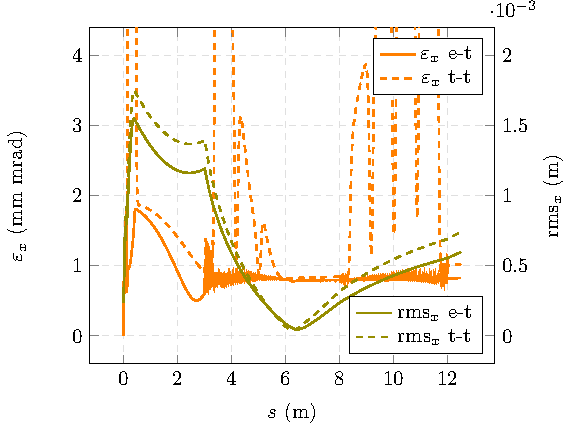
\includegraphics[width=0.9\linewidth]{Report/iff_plot_emrms_ettt}
  \caption{Comparison 3D-tracker versus envelope-tracker in case for rms$_{x}$
    and $\varepsilon_{x}$.}
  \label{fig:et-vs-tt}
\end{figure}

%\subsection{IW2: Inverse Problem}

%In order to find cross correlations we try to solve the inverse problem
  %(15) -- (23)
%%
%\begin{align}
  %\text{min}  \quad & \sqrt{\frac{1}{N} \sum \left( \text{rmx}_{x,s} -
                      %\text{m}_{x,s} \right)^2 } \text{,}\\
              %\quad & \sqrt{\frac{1}{N} \sum \left( \text{rmx}_{y,s} -
                      %\text{m}_{y,s} \right)^2 } \text{,}\\
              %\quad & \sqrt{\frac{1}{N} \sum \left( \text{rmx}_{z,s} -
                      %\text{m}_{z,s} \right)^2 } \\
  %\text{s.t.} \quad & -0.95 \leq \text{R52} \leq -0.65 \label{eq:iw2:fistdvar}\\
              %\quad & -0.90 \leq \text{R61} \leq -0.50 \\
              %\quad & 0.0   \leq \text{R62} \leq 0.20 \\
              %\quad & 0.25 \leq \text{CORR}_x \leq 0.65 \\
              %\quad & 0.55 \leq \text{CORR}_y \leq 0.95 \\
              %\quad & 0.10 \leq \text{CORR}_z \leq 0.50 \label{eq:iw2:lastdvar} \text{.}
%\end{align}
%%
%We try to match the beam to measurements from the real machine by minimizing
  %the sum of $N$ squared measurement ($m_{d,s}$ at a given position
  %$s$) errors for rmx beam size in each dimensions.
%The design variables (\ref{eq:iw2:fistdvar}) - (\ref{eq:iw2:lastdvar}) define
  %the correlation matrix used when generating particles, e.g., R51, R52, R61,
  %R62 describe limits of correlations between planes.
%The initial Binomial distribution (with $m = ?$) has the form
%%
%\begin{equation*}
  %\frac{1}{2\pi\sigma_x\sigma_y}exp(-\frac{x^2}{2\sigma_x^2}
  %-\frac{y^2}{2\sigma_y^2})
  %\text{.}
%\end{equation*}
%%

%Since these correlations cannot be measured we get the real values by solving
  %the inverse problem mentioned above.

%Currently we run the simulations on a low resolution space charge grid ($8
  %\times 8 \times 8$) as a proof of concept.
%In a next step a simple Python script would be applied to iteratively rerun
  %the optimizer with increasing space-charge resolution when the limits of the
  %design variables are narrow enough (iteratively diminishing search space).
%\subsection{IW2: Inverse Problem}

%In order to find cross correlations we try to solve the inverse problem
  %(15) -- (23)
%%
%\begin{align}
  %\text{min}  \quad & \sqrt{\frac{1}{N} \sum \left( \text{rmx}_{x,s} -
                      %\text{m}_{x,s} \right)^2 } \text{,}\\
              %\quad & \sqrt{\frac{1}{N} \sum \left( \text{rmx}_{y,s} -
                      %\text{m}_{y,s} \right)^2 } \text{,}\\
              %\quad & \sqrt{\frac{1}{N} \sum \left( \text{rmx}_{z,s} -
                      %\text{m}_{z,s} \right)^2 } \\
  %\text{s.t.} \quad & -0.95 \leq \text{R52} \leq -0.65 \label{eq:iw2:fistdvar}\\
              %\quad & -0.90 \leq \text{R61} \leq -0.50 \\
              %\quad & 0.0   \leq \text{R62} \leq 0.20 \\
              %\quad & 0.25 \leq \text{CORR}_x \leq 0.65 \\
              %\quad & 0.55 \leq \text{CORR}_y \leq 0.95 \\
              %\quad & 0.10 \leq \text{CORR}_z \leq 0.50 \label{eq:iw2:lastdvar} \text{.}
%\end{align}
%%
%We try to match the beam to measurements from the real machine by minimizing
  %the sum of $N$ squared measurement ($m_{d,s}$ at a given position
  %$s$) errors for rmx beam size in each dimensions.
%The design variables (\ref{eq:iw2:fistdvar}) - (\ref{eq:iw2:lastdvar}) define
  %the correlation matrix used when generating particles, e.g., R51, R52, R61,
  %R62 describe limits of correlations between planes.
%The initial Binomial distribution (with $m = ?$) has the form
%%
%\begin{equation*}
  %\frac{1}{2\pi\sigma_x\sigma_y}exp(-\frac{x^2}{2\sigma_x^2}
  %-\frac{y^2}{2\sigma_y^2})
  %\text{.}
%\end{equation*}
%%

%Since these correlations cannot be measured we get the real values by solving
  %the inverse problem mentioned above.

%Currently we run the simulations on a low resolution space charge grid ($8
  %\times 8 \times 8$) as a proof of concept.
%In a next step a simple Python script would be applied to iteratively rerun
  %the optimizer with increasing space-charge resolution when the limits of the
  %design variables are narrow enough (iteratively diminishing search space). 
%\vspace{-7em}
\subsection{AWA Photoinjector Optimization}
Next we apply the optimization framework to the high charge beam line at the AWA, 
which consists of an rf photocathode gun, two solenoids, six linear accelerating cavities, 
followed by four quadrupoles and a stripline kicker, as shown in Fig. \ref{awa-pic}. 
Portions of this beam line served as the injector for Two Beam 
Acceleration (TBA) experiments in the past [X1], and will be used for 
similar experiments in the future [X2]. Main constraints on prior experimental 
results were the beam size and emittance as the beam passed through small aperture 
wakefield structures located after the quadrupoles. 
In an attempt to maximize charge transmission in upcoming experiments
we optimize several parameters in the gun and quadrupole leading into the 
TBA section of the beam line.
%\vspace{-1em}

\begin{figure}
	\centering
	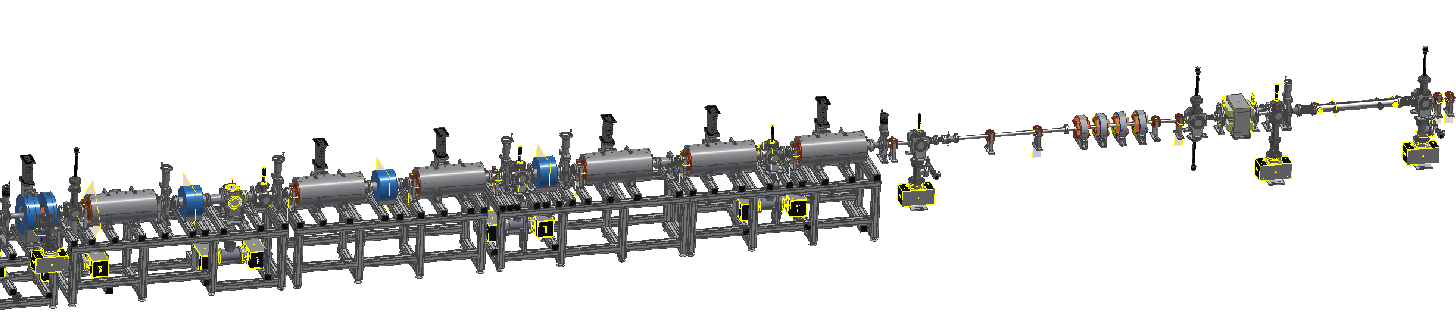
\includegraphics[width=0.9\linewidth]{Report/awa-drawing}
	\caption{High charge beam line layout at the AWA.}
	\label{awa-pic}
\end{figure}

\vspace{-1em}
Compared to the Ferrario experiment in Section \ref{ferrario}, 
we increase the number of design variables and objectives by a factor of two.
The problem is also less predictable, due to the increased number of design variables
and nonlinear effects such as space charge, there is not a definite idea
before hand where the Pareto front will fall. This work is also meaningful in that
it will guide future operations at the AWA.

\begin{align}
\text{min}  \quad & \text{rms}_{x, s_1}, \quad \text{rms}_{x, s_2} \label{eq:awa:p1}\\
& \text{rms}_{s, s_1}, \quad \text{rms}_{s, s_2} \label{eq:awa:p2}\\
& \varepsilon_{x,s_1}, \quad \varepsilon_{x,s_2} \label{eq:awa:p3} \\
& dE \label{eq:awa:p4} \\
\text{subject to} \quad & q = 40 \left[\text{nC}\right] \label{eq:awa:firstconstr}\\
\quad & \text{Volt}_{\text{Gun}} = 64\left[\text{MV/m}\right] \label{eq:awa:lastconstr}\\
\quad & \text{Volt}_{\text{Linac}} = 24-25\left[\text{MV/m}\right] \\
\quad & \sigma_x = \sigma_y = 9 \left[\text{mm}\right] \label{eq:awa:firstdvar}\\
\quad & \phi_{\text{linac}} =0 \label{eq:awa:lastdvar}
\end{align}

The first four objectives minimize the transverse ($rms_x$) and longitudinal ($rms_s$) 
beam sizes at two locations of interest in the beam line ($s_1$,$s_2$). 
These are the longitudinal positions at the entrance of the kicker and 
$1[\text{m}]$ after the exit of the kicker. The beam size needs to be minimized
here to prevent scraping and ensure transmission through the wakefield structures 
following the kicker. The next two objectives (\ref{eq:awa:p4}) minimize the 
transverse emittance, which favors less divergence in the beam and reduces 
emittance growth during transport. The last objective (\ref{eq:awa:p4}), 
minimizes energy spread in the bunch at the entrance of the kicker, $s_1$.  
This helps reduce emittance and beam size growth in the kicker.  
Equations (\ref{eq:awa:firstconstr}) to
(\ref{eq:awa:lastdvar}) define the charge, gun voltage, linac voltages, 
laser radius and linac cavity phases. These are parameters in the simulation 
that must be defined, but do not vary during the optimization.

%\vspace{-1em}
As introduced in Section \ref{ferrario}, we define the AWA optimization problem 
objectives, and design variables in the OPAL input file as shown in
the following code: %equations (\ref{eq:awa:p1}) to (\ref{eq:awa:lastdvar}). 

\vspace{0.2cm}
{\footnotesize \begin{verbatim}
	// Gun variables
	dv0: DVAR, VARIABLE="IBF",    LOWERBOUND=350.0, UPPERBOUND=500.0;
	dv1: DVAR, VARIABLE="IM",     LOWERBOUND=170.0, UPPERBOUND=260.0;
	dv2: DVAR, VARIABLE="GPHASE", LOWERBOUND=-30.0, UPPERBOUND=0.0;
	dv3: DVAR, VARIABLE="FWHM",   LOWERBOUND=1.5,   UPPERBOUND=10.0;
	
	// Quad variables
	dv4: DVAR, VARIABLE="KQ1", LOWERBOUND=-8.0, UPPERBOUND=8.0;
	dv5: DVAR, VARIABLE="KQ2", LOWERBOUND=-8.0, UPPERBOUND=8.0;
	dv6: DVAR, VARIABLE="KQ3", LOWERBOUND=-8.0, UPPERBOUND=8.0;
	dv7: DVAR, VARIABLE="KQ4", LOWERBOUND=-8.0, UPPERBOUND=8.0;
	
	// Objectives
	rmss1:  OBJECTIVE,EXPR="fabs(statVariableAt('rms_s',16.45))";
	rmsx1:  OBJECTIVE,EXPR="fabs(statVariableAt('rms_x',16.45))";
	emitx1: OBJECTIVE,EXPR="fabs(statVariableAt('emit_x',16.45))";
	de1:    OBJECTIVE,EXPR="fabs(statVariableAt('dE',16.45))";	
	rmss2:  OBJECTIVE,EXPR="fabs(statVariableAt('rms_s',18.45))";
	rmsx2:  OBJECTIVE,EXPR="fabs(statVariableAt('rms_x',18.45))";
	emitx2: OBJECTIVE,EXPR="fabs(statVariableAt('emit_x',18.45))";

	\end{verbatim}}
\vspace{0.2cm}

Design variables include the currents in two gun solenoids (IBF and IM), 
the gun phase (GPHASE), the laser longitudinal full width half max (FWHM), 
and four quadrupole strengths (KQ1-KQ2). The objectives include
beam size, emittance, and energy spread as
defined in Eqs. (\ref{eq:awa:p1}) to (\ref{eq:awa:p4}). 
The s location at the entrance of the kicker is $s_1=16.45[\text{m}]$, 
and the s location of interest after the kicker is $s_1=18.45[\text{m}]$. 

All simulations for this experiment were carried out on Bebop a
high performance computing (HPC)
cluster provided by the Laboratory Computing Resource Center (LCRC)
at Argonne National Laboratory (ANL). We used Intel Knights Landing 
(KNL) processors at 1.3 GHz with 128 GB of memory 
and 64 cores per node. There are 352 compute nodes available on 
Bebop, with a total of 22,528 cores. 
This allows for very large optimization jobs, like the AWA case.

OPAL was used as the forward solver, and a study on time step and 
number of particles was done to reduce the time to simulation while 
maintaining the physics of interest. All jobs were run and compared 
on 8 cores each, which allowed 8 jobs per node on the KNL.
The grid size was $16 \times 16 \times 32$, 
and parallelized in the x and y directions.
After comparing several options we choose ten thousand particles 
in combination with adjusting the time step near sensitive elements 
(i.e. quadurpoles, kicker). 
The resulting simulations are low fidelity, but closely approximate 
the mid fidelity simulations for metrics of interest, as shown in 
Fig. \ref{tstep}.

\begin{figure}
	\centering
	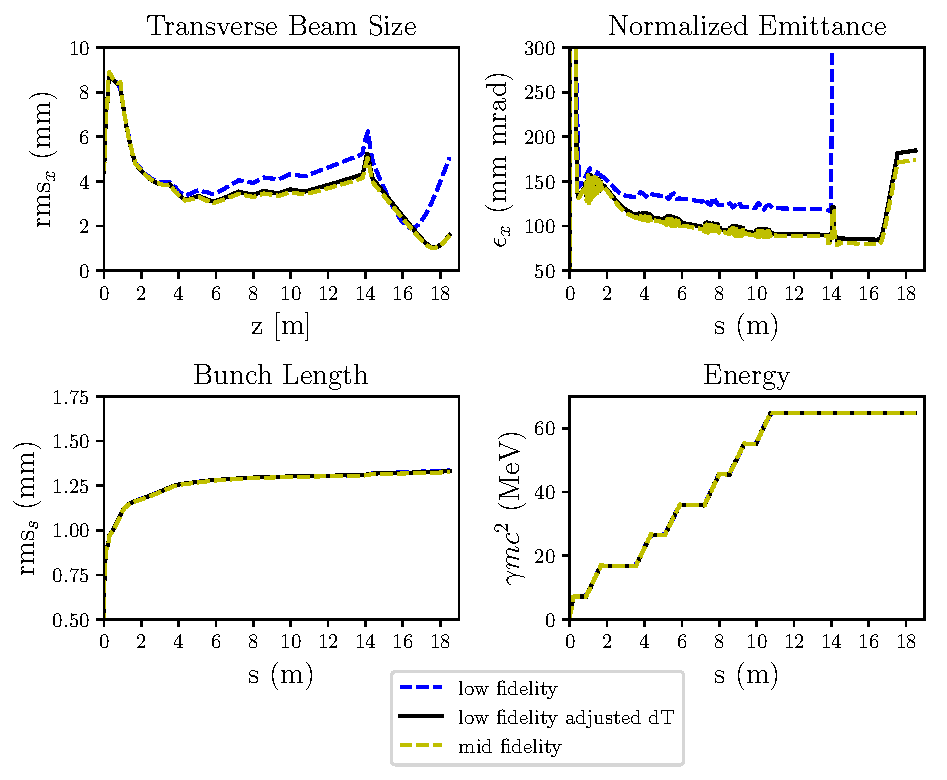
\includegraphics[width=0.8\linewidth]{Report/timestep_comparison}
	\caption{Comparison of different fidelity models.}
	\label{tstep}
\end{figure}


\begin{table}%[h!]
	\begin{center}
		\caption{Low and mid fidelity simulation parameters.}
		\label{fidelity}

		\begin{tabular*}{\textwidth}{l @{\extracolsep{\fill}} C c D }
			\hline\noalign{\smallskip}
			& Number of particles & dT (seconds) & Time to simulation (minutes)\\
			\noalign{\smallskip}\hline\noalign{\smallskip}
			low fidelity  			&  10,000   & $5 \times10^{-11}$  &  2.6 \\
			adjusted low fidelity  	&  10,000   & $2 \times 10^{-12}$, $1 \times 10^{-11}$ & 1.6 \\
			mid fidelity 			&  100,000  & $1 \times 10^{-12}$ &  18\\
			\noalign{\smallskip}\hline
		\end{tabular*}
	\end{center}
\end{table}

\subsubsection{AWA Optimization Results}


